
\begin{figure}
   \centering
   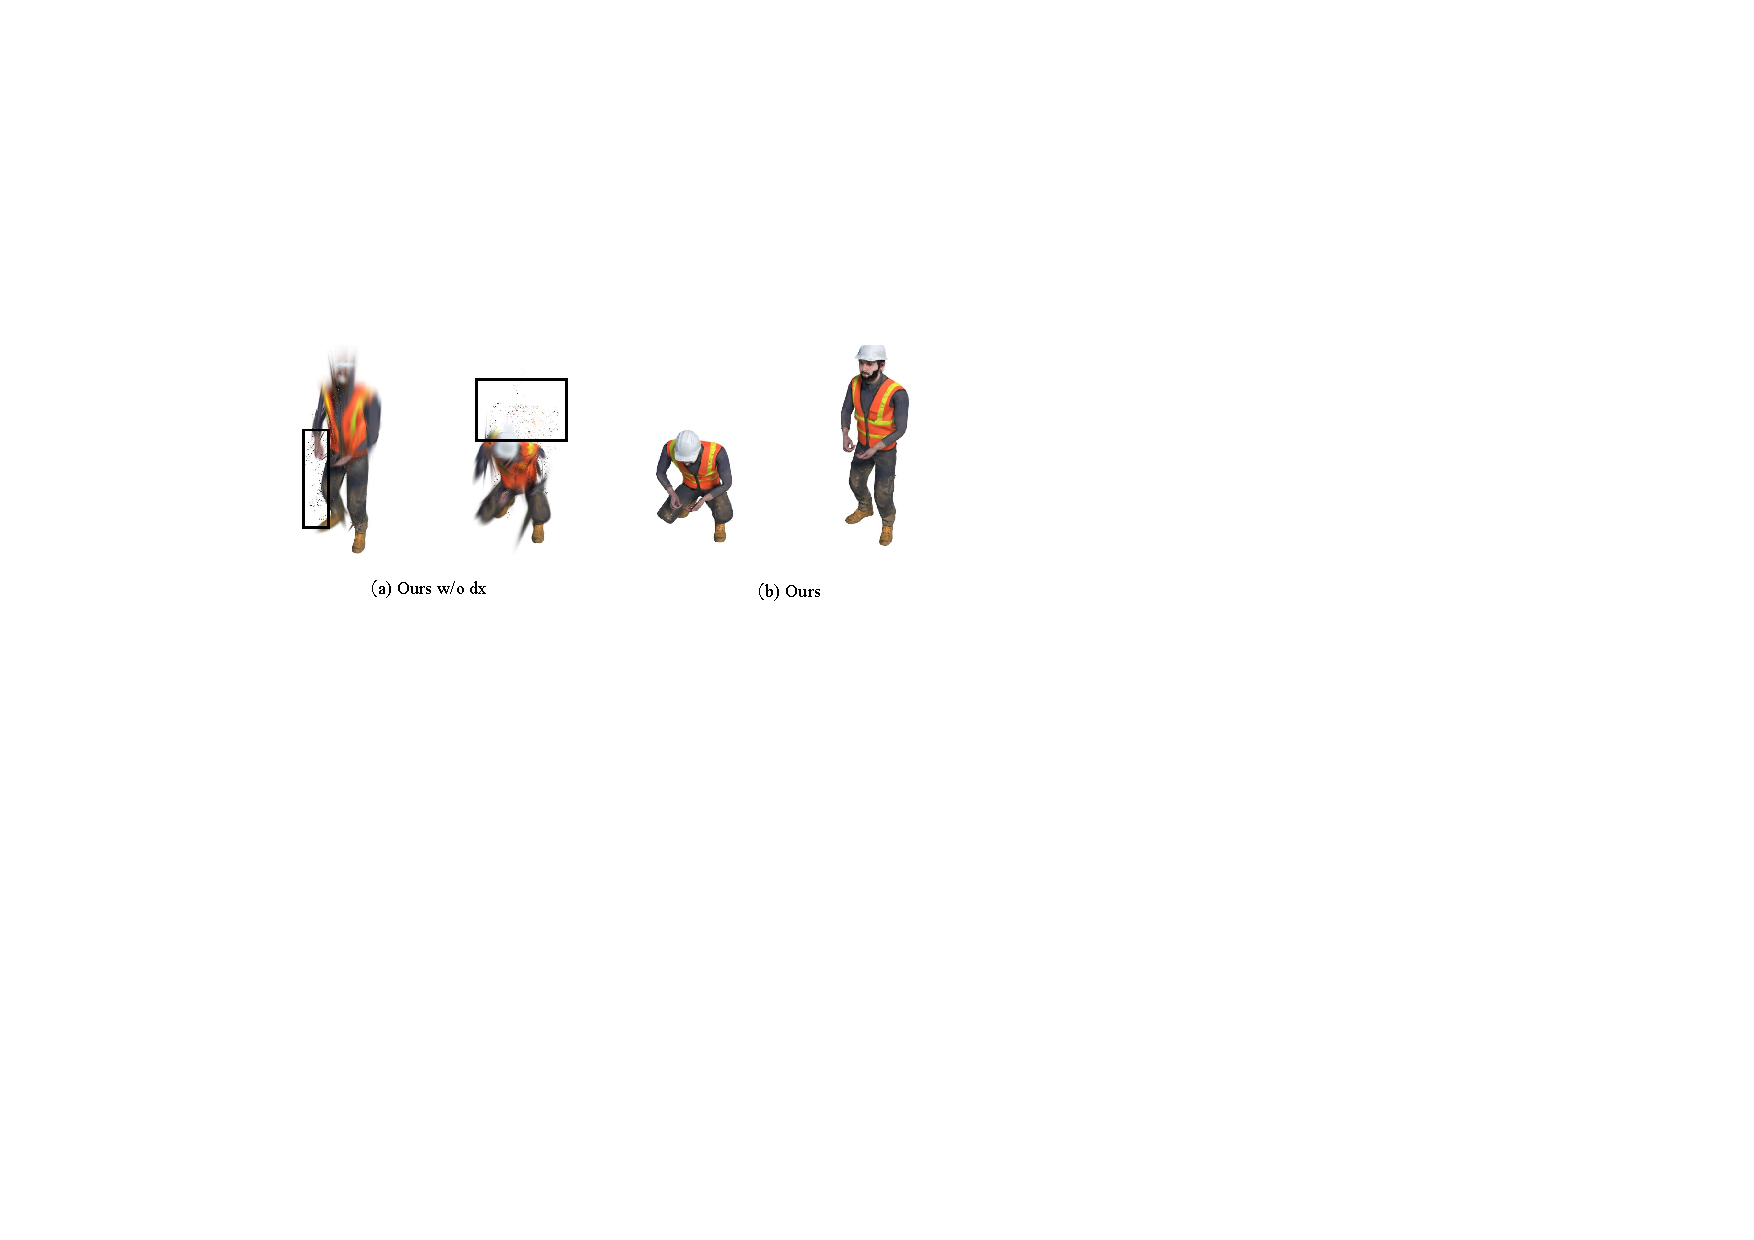
\includegraphics[width=\linewidth]{fig/no_dx_vis.pdf}
   \caption{Visualization of ablation study about $\phi_x$.}
    \label{fig:no_dx_vis}
\end{figure}

\begin{figure*}
   \centering
   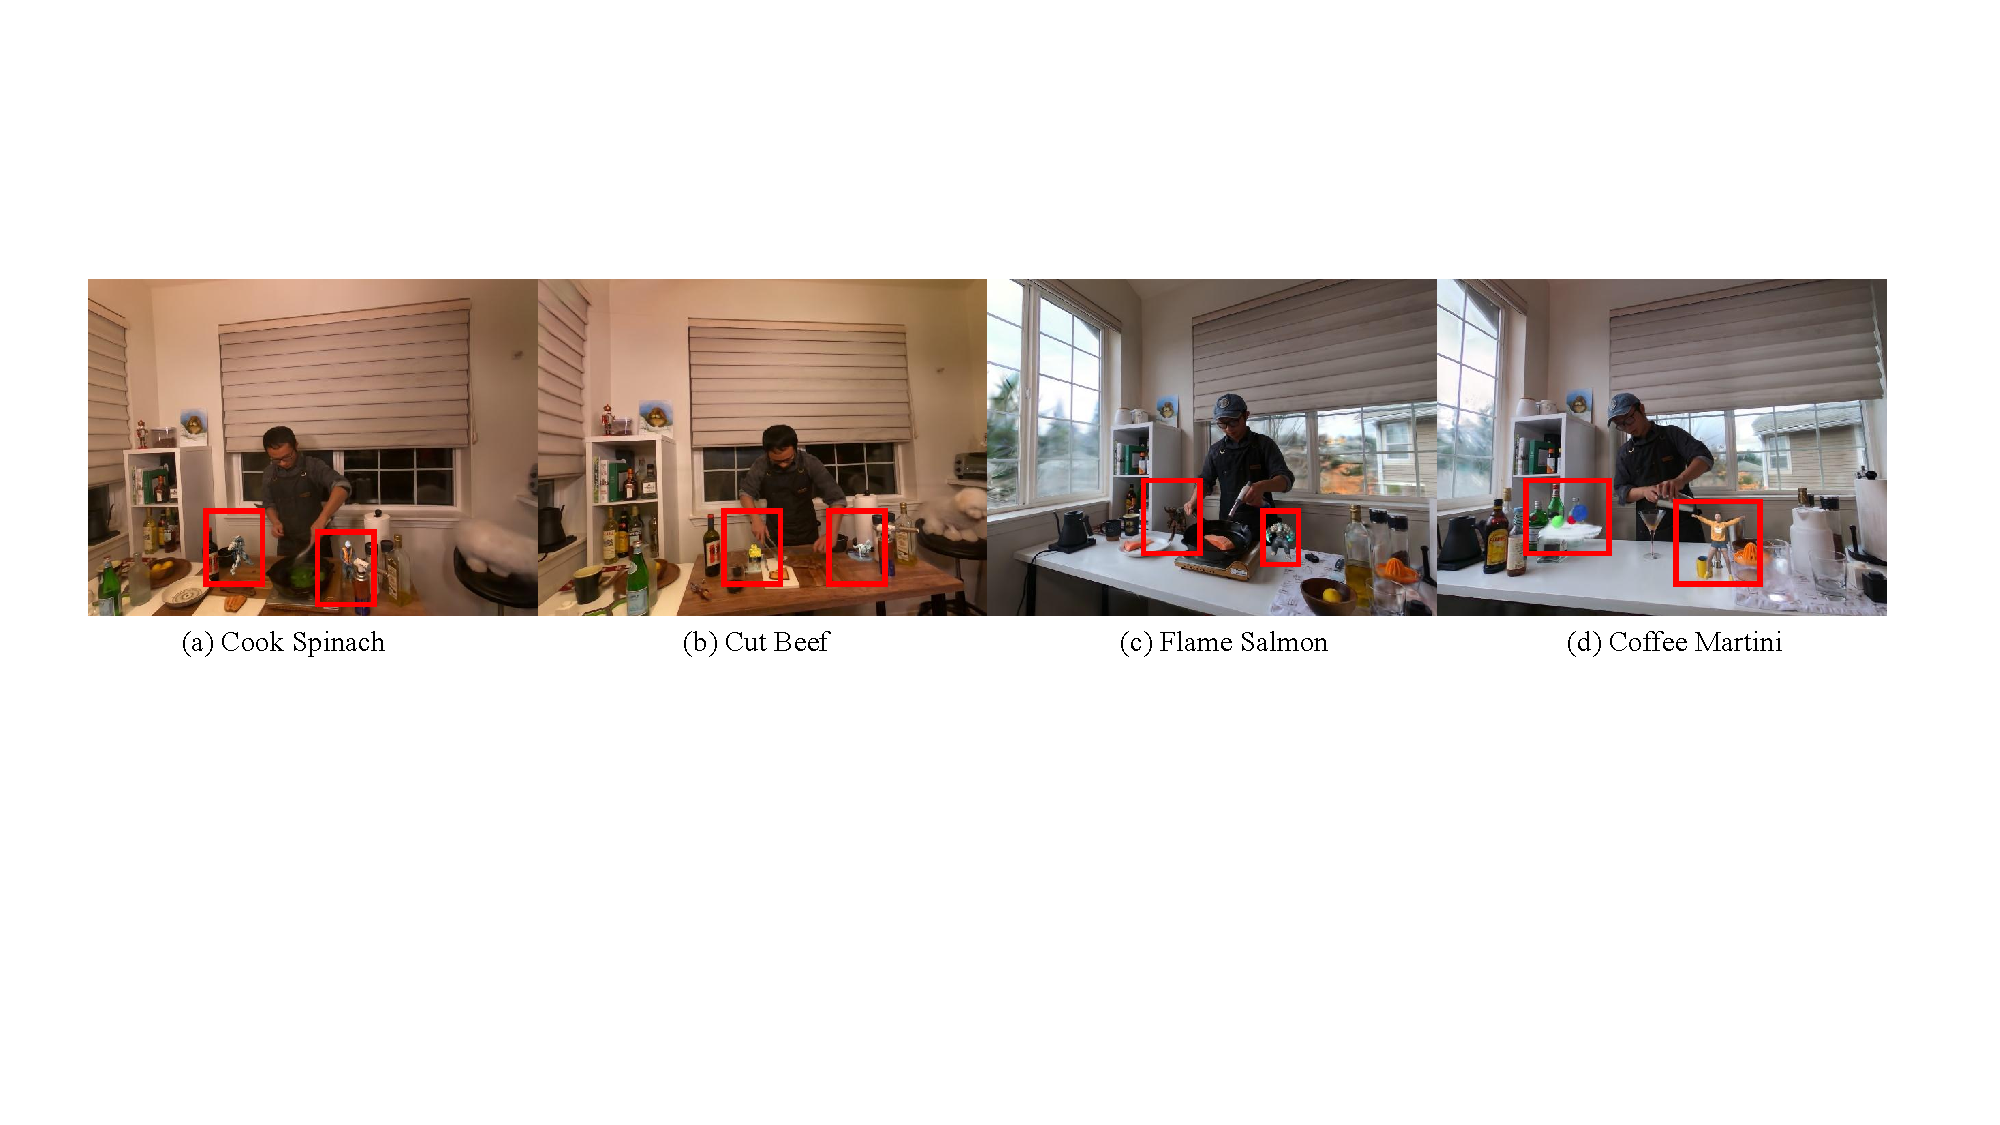
\includegraphics[width=1.0\linewidth]{fig/editing_supp.pdf}
   \caption{More visualization of composition in 4D Gaussians. (a) Composition with Punch and Standup. (b) Composition with Lego and Trex. (c) Composition with Hellwarrior and Mutant. (d) Composition with Bouncingballs and Jumpingjacks.}
    \label{fig:editing_supp}
\end{figure*}
\begin{figure}
   \centering
   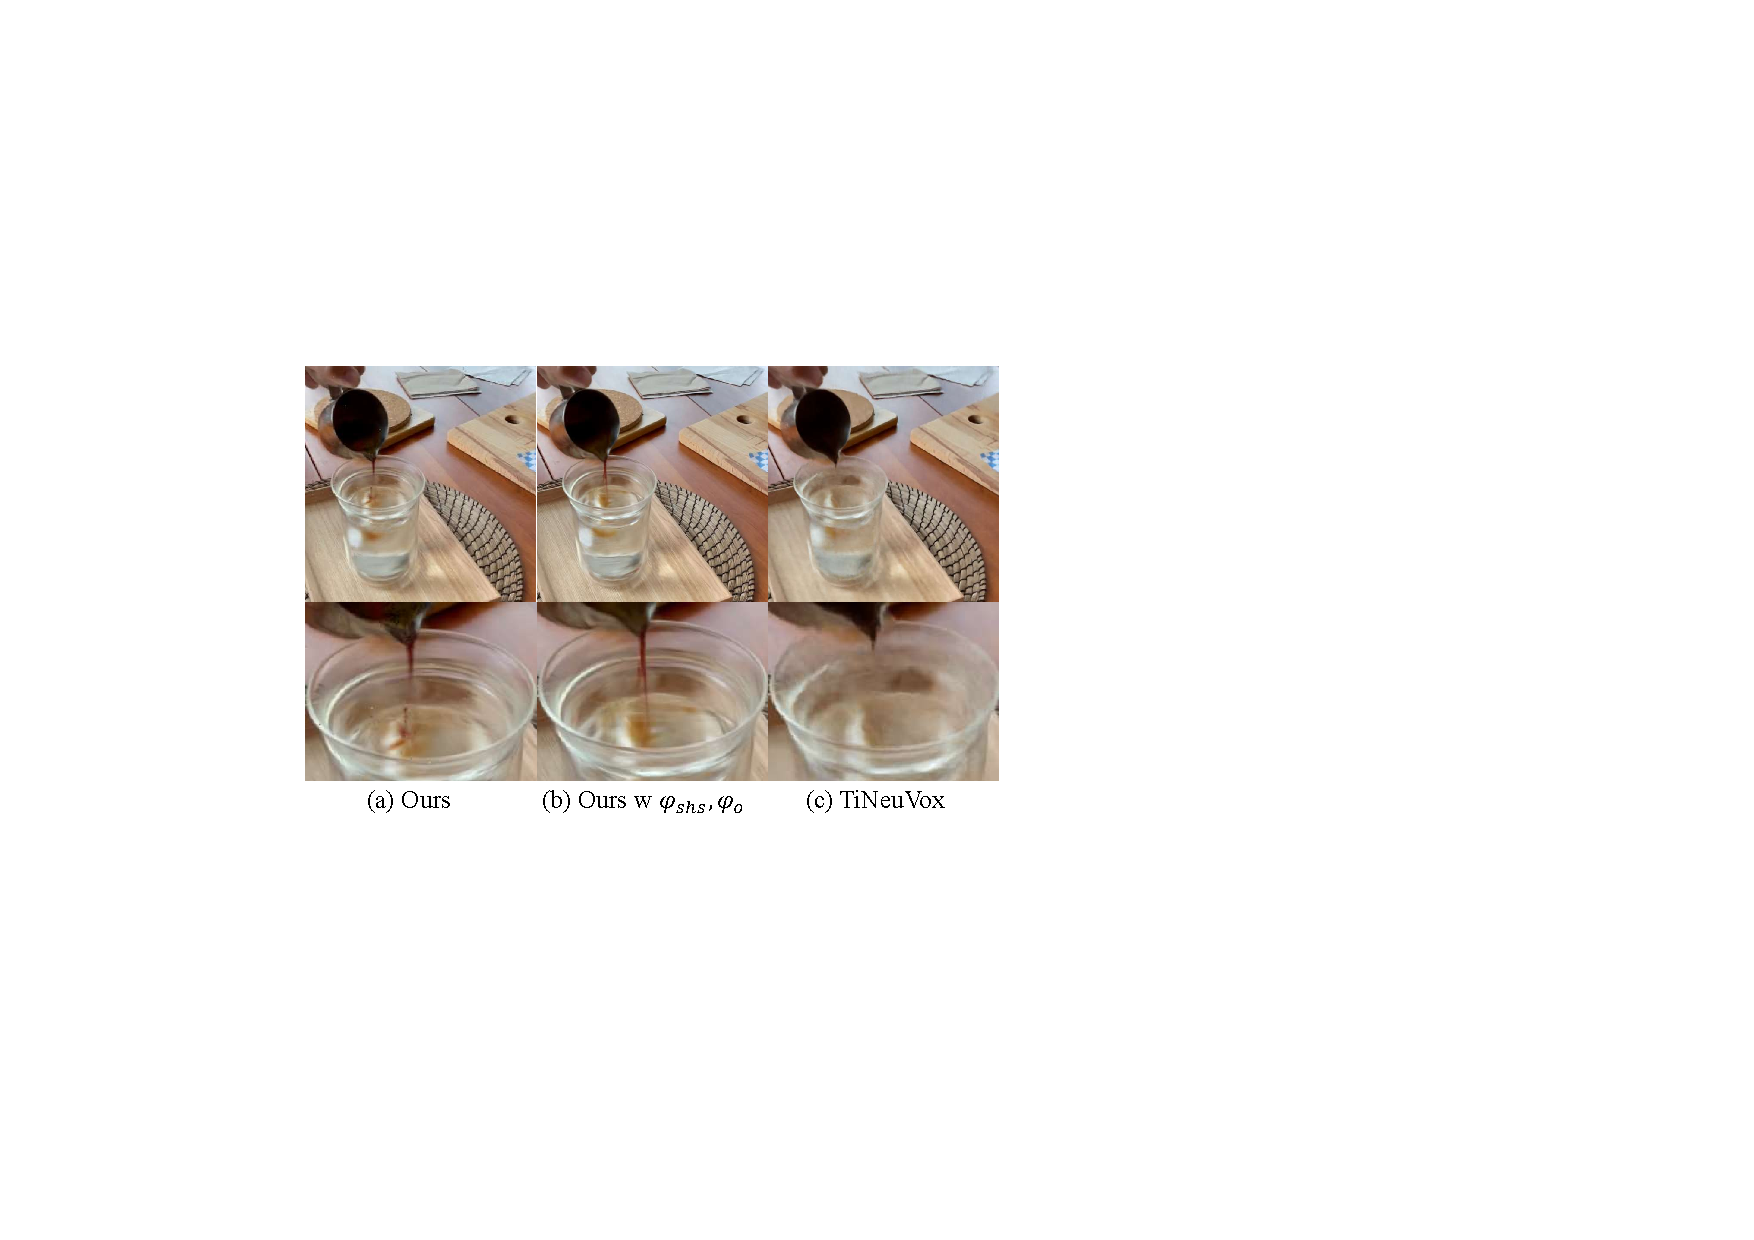
\includegraphics[width=1.0\linewidth]{fig/ab_dshs.pdf}
   \caption{Visualization of ablation study in $\phi_{\mathcal{C}}$ and $\phi_{\mathcal{\alpha}}$ comparing with TiNeuVox~\cite{tineuvox}.}
    \label{fig:ab_dshs}
\end{figure}
\begin{figure*}
   \centering
   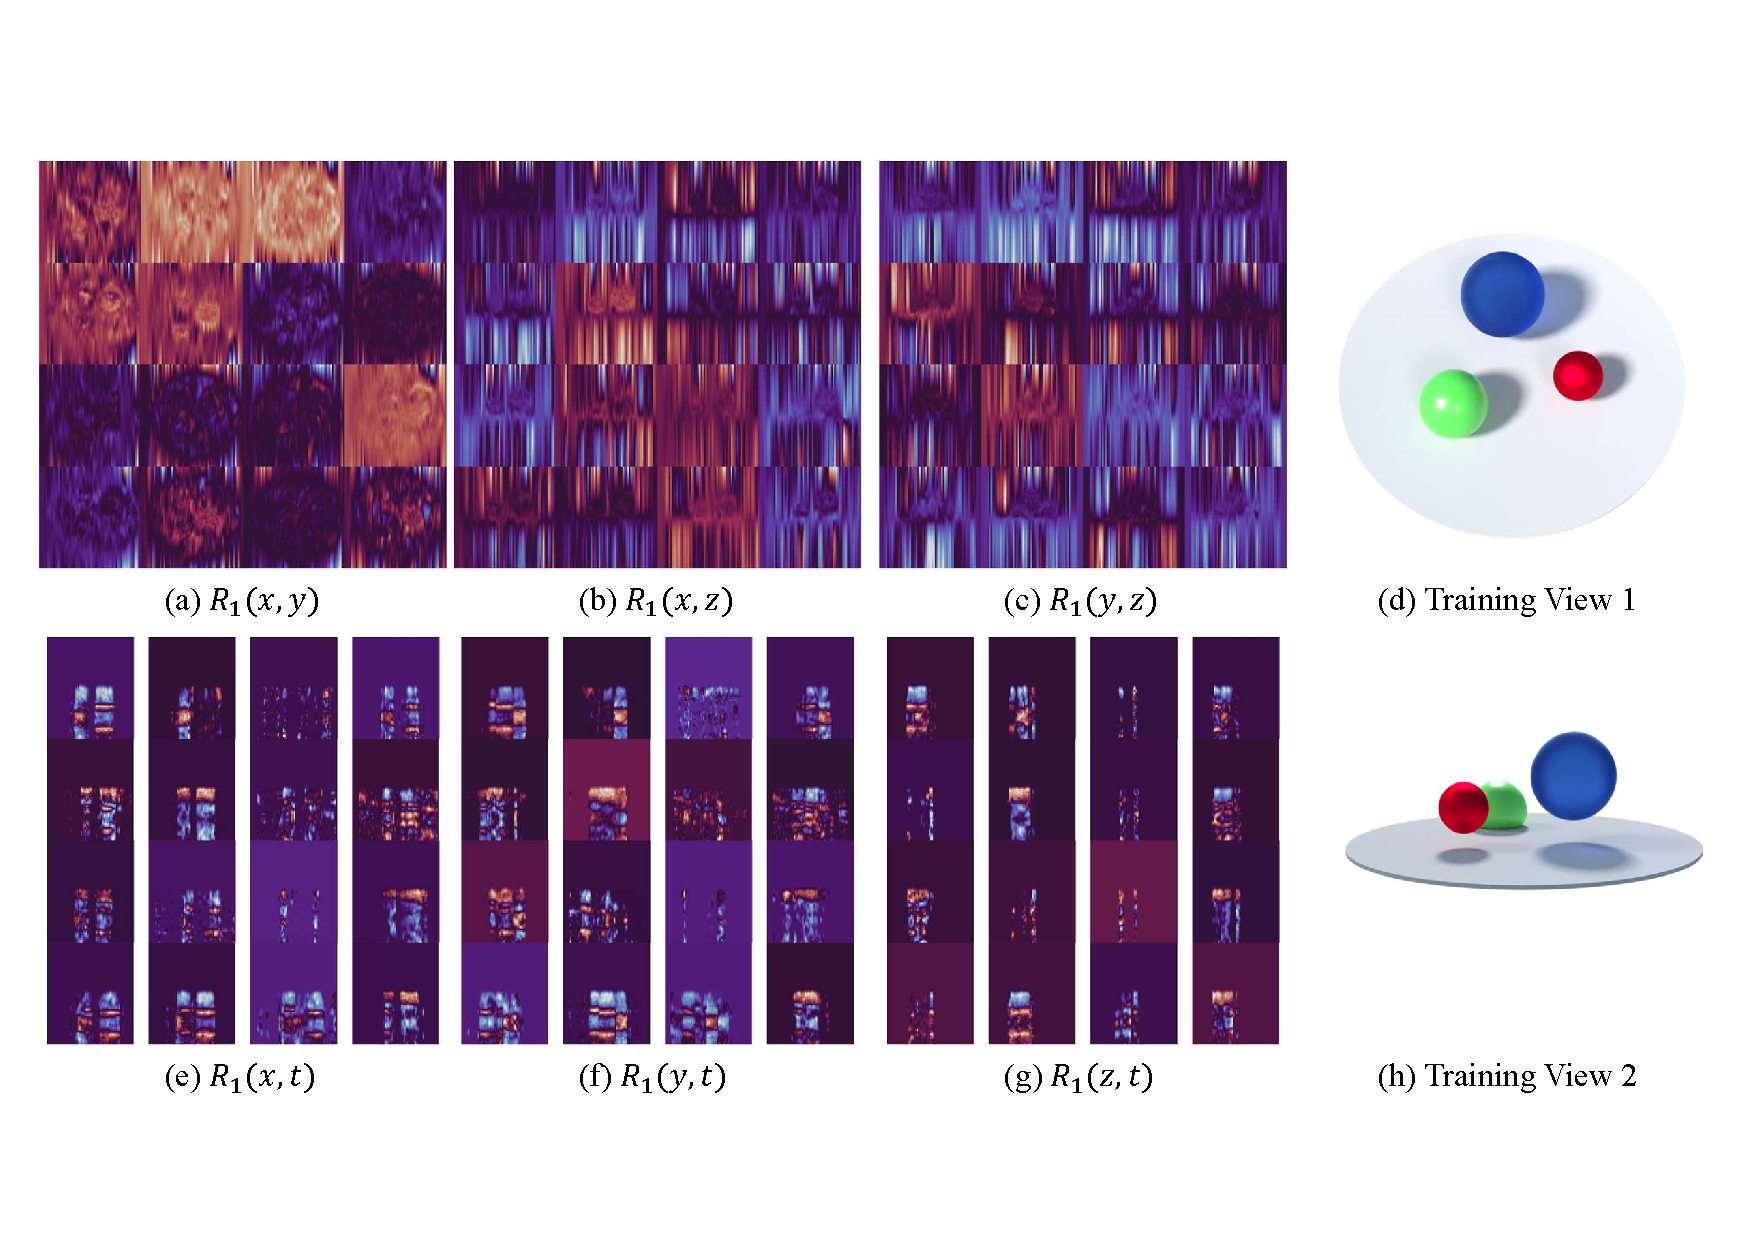
\includegraphics[width=1.0\linewidth]{fig/grid_features2.pdf}
   \caption{More visualization of the HexPlane voxel grids $R(i,j)$ in bouncing balls. (a)-(c), (e)-(f) stand for visualization of $R_1(i,j)$, where grids resolution equals to 64$\times$64.}
    \label{fig:grid_feature_vis_supp}
\end{figure*}



\begin{figure}
   \centering
   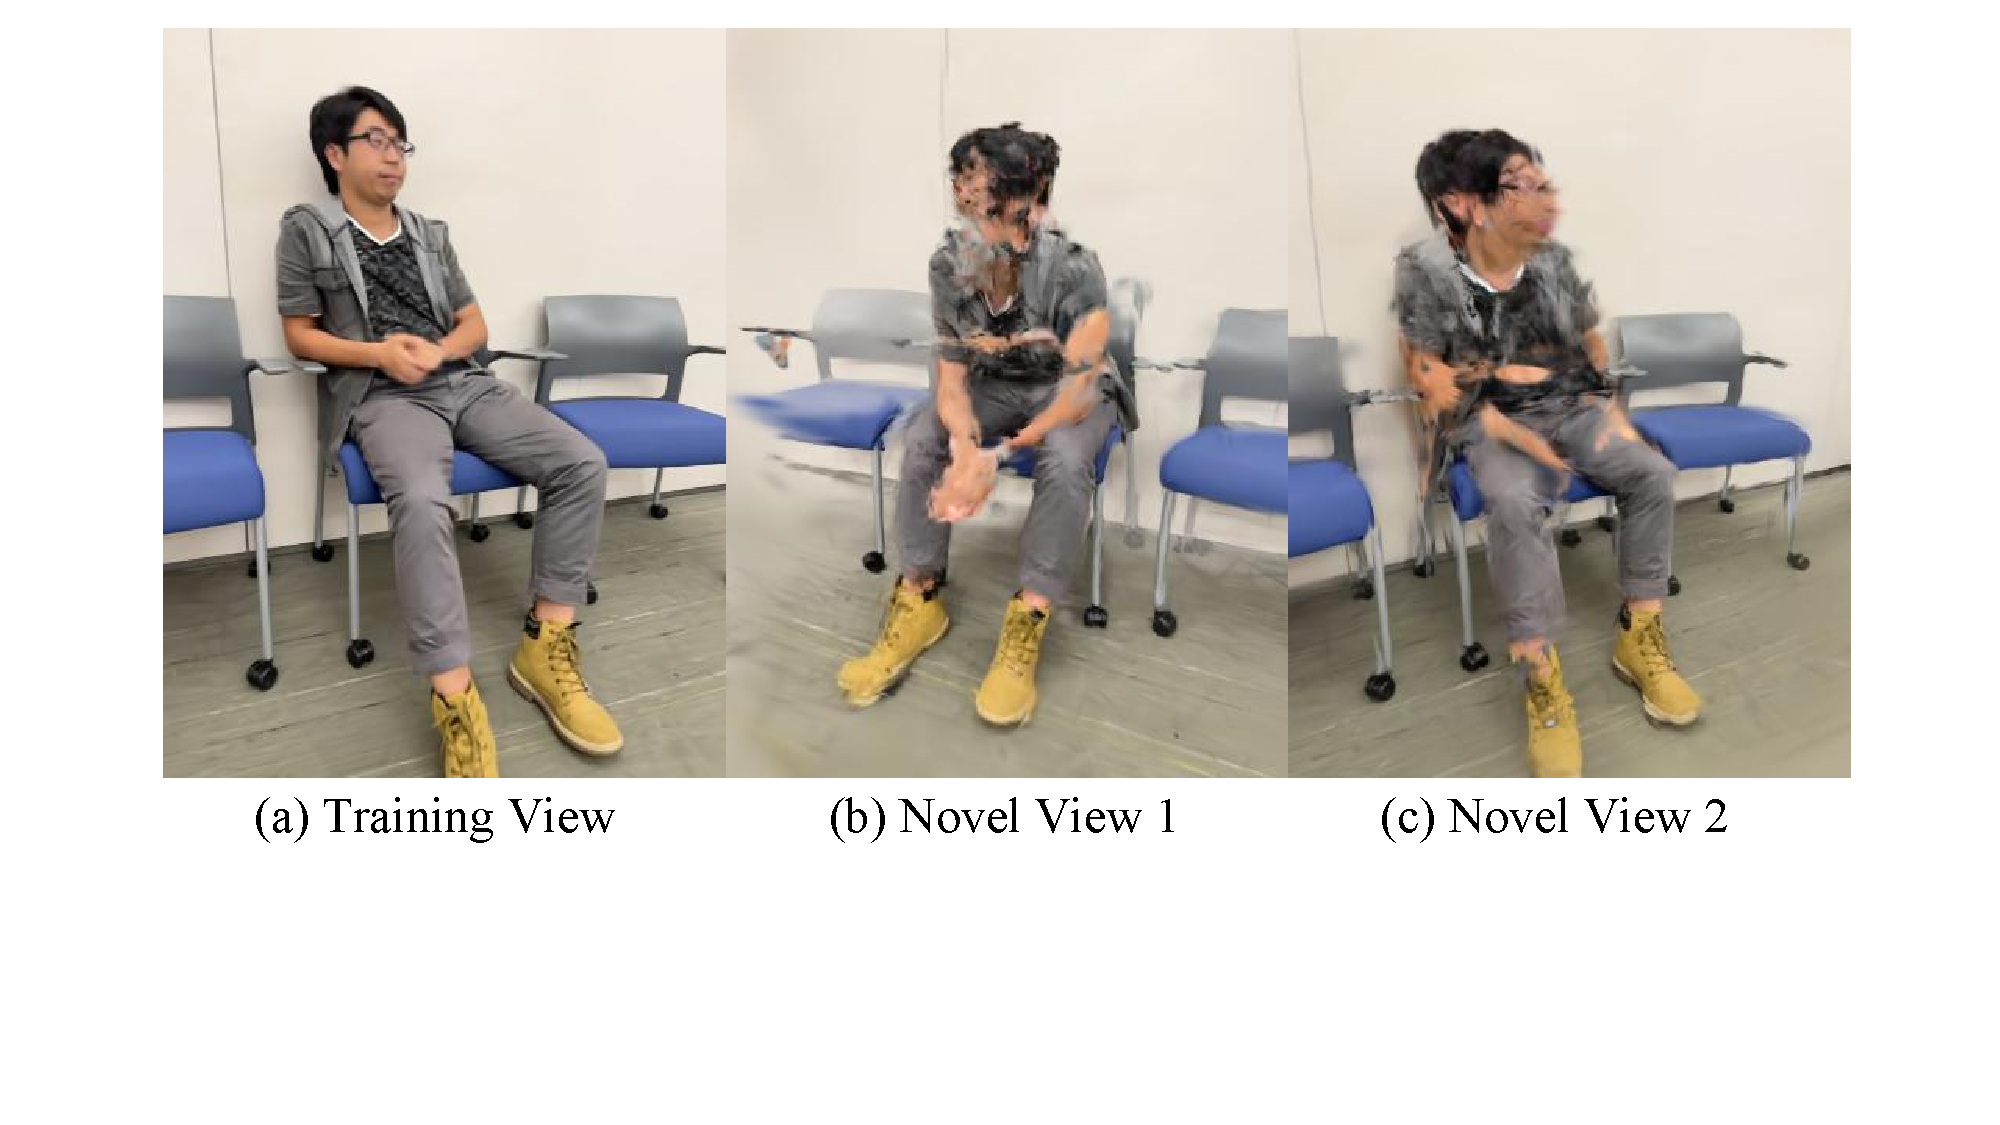
\includegraphics[width=1.0\linewidth]{fig/dycheck.pdf}
   \caption{Novel view rendering results in the iPhone datasets~\cite{dycheck}.}
    \label{fig:dycheck_supp}
\end{figure}

\begin{figure}
   \centering
   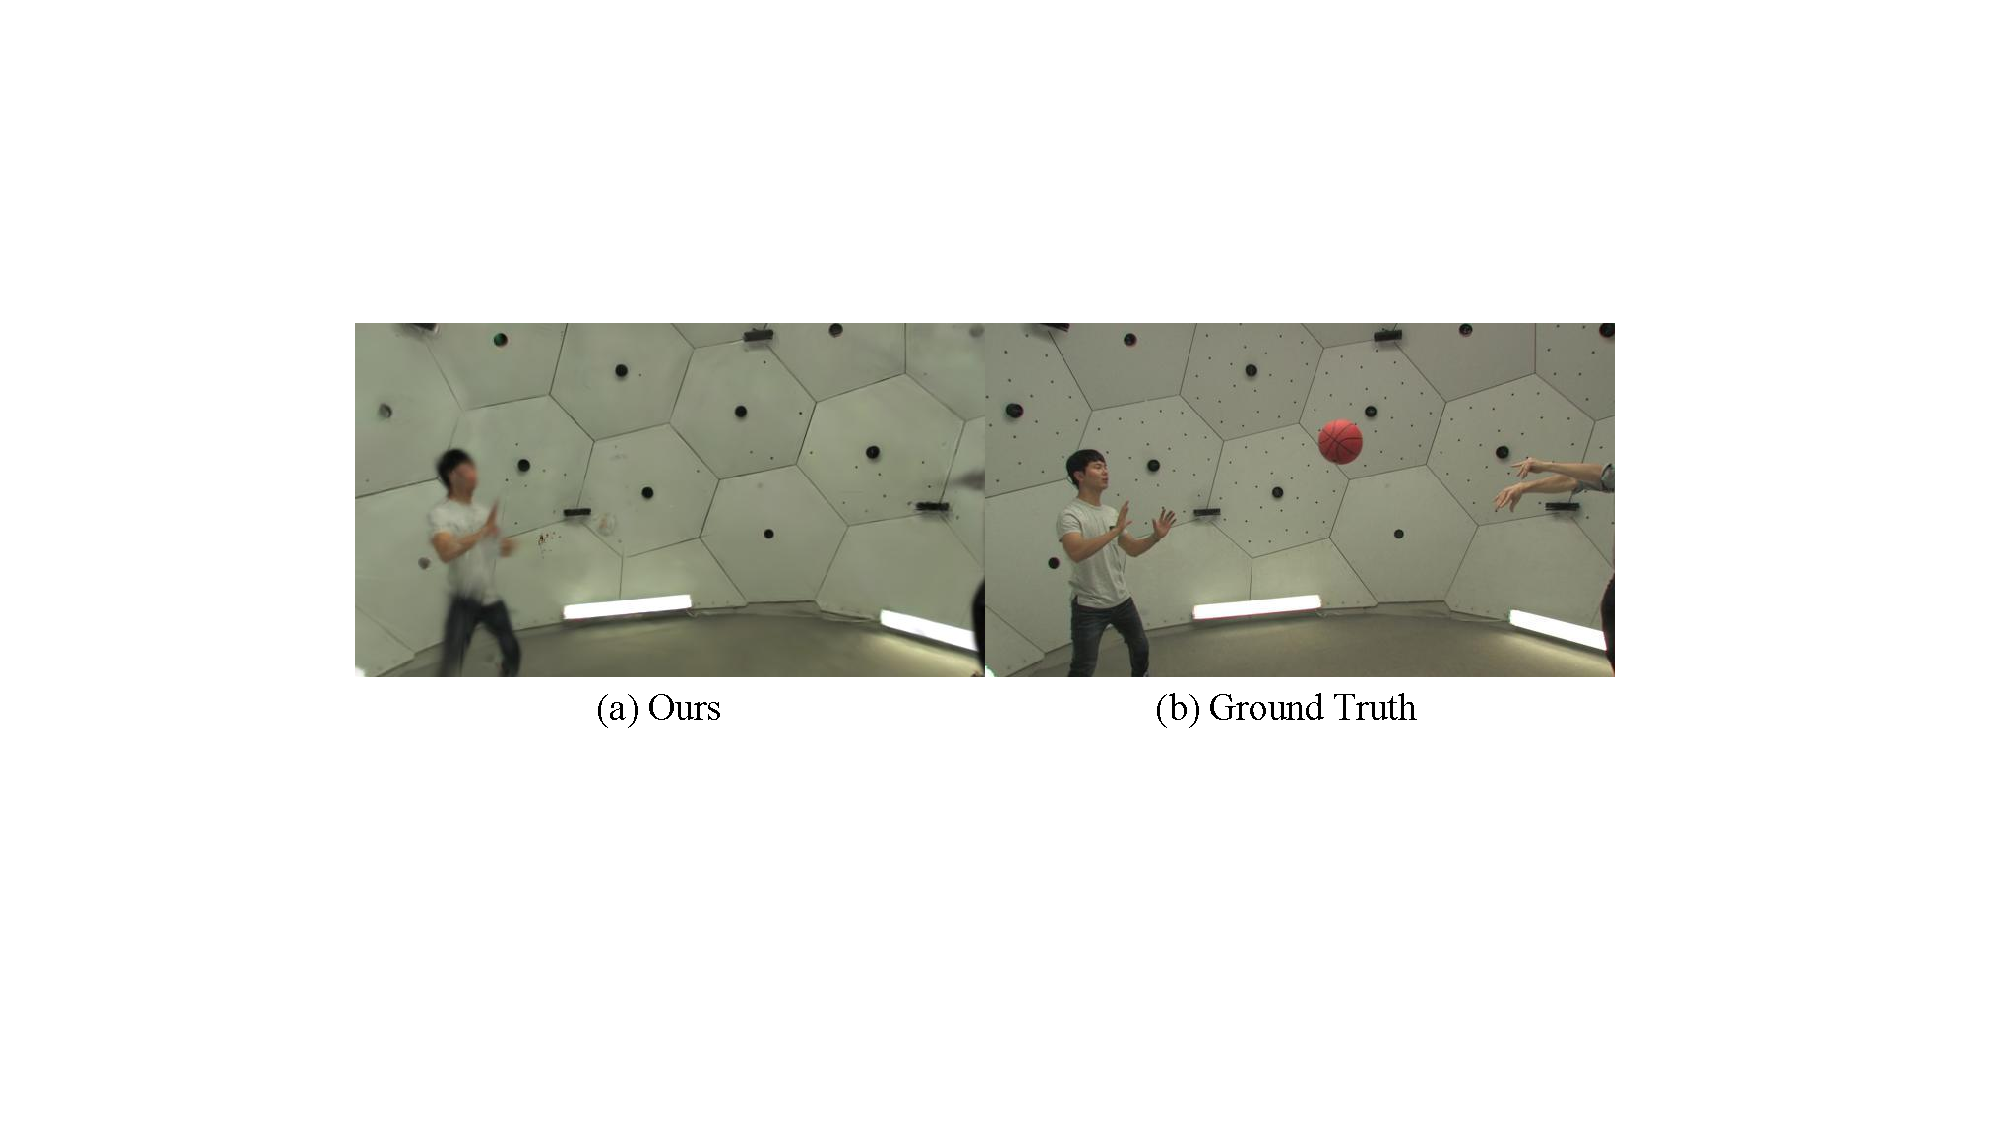
\includegraphics[width=1.0\linewidth]{fig/sports.pdf}
   \caption{Rendering results on sports dataset~\cite{joo2015panopticstudio} also used in Dynamic3DGS~\cite{dynamic3dgs}.}
    \label{fig:sports_supp}
\end{figure}

\begin{figure}
   \centering
   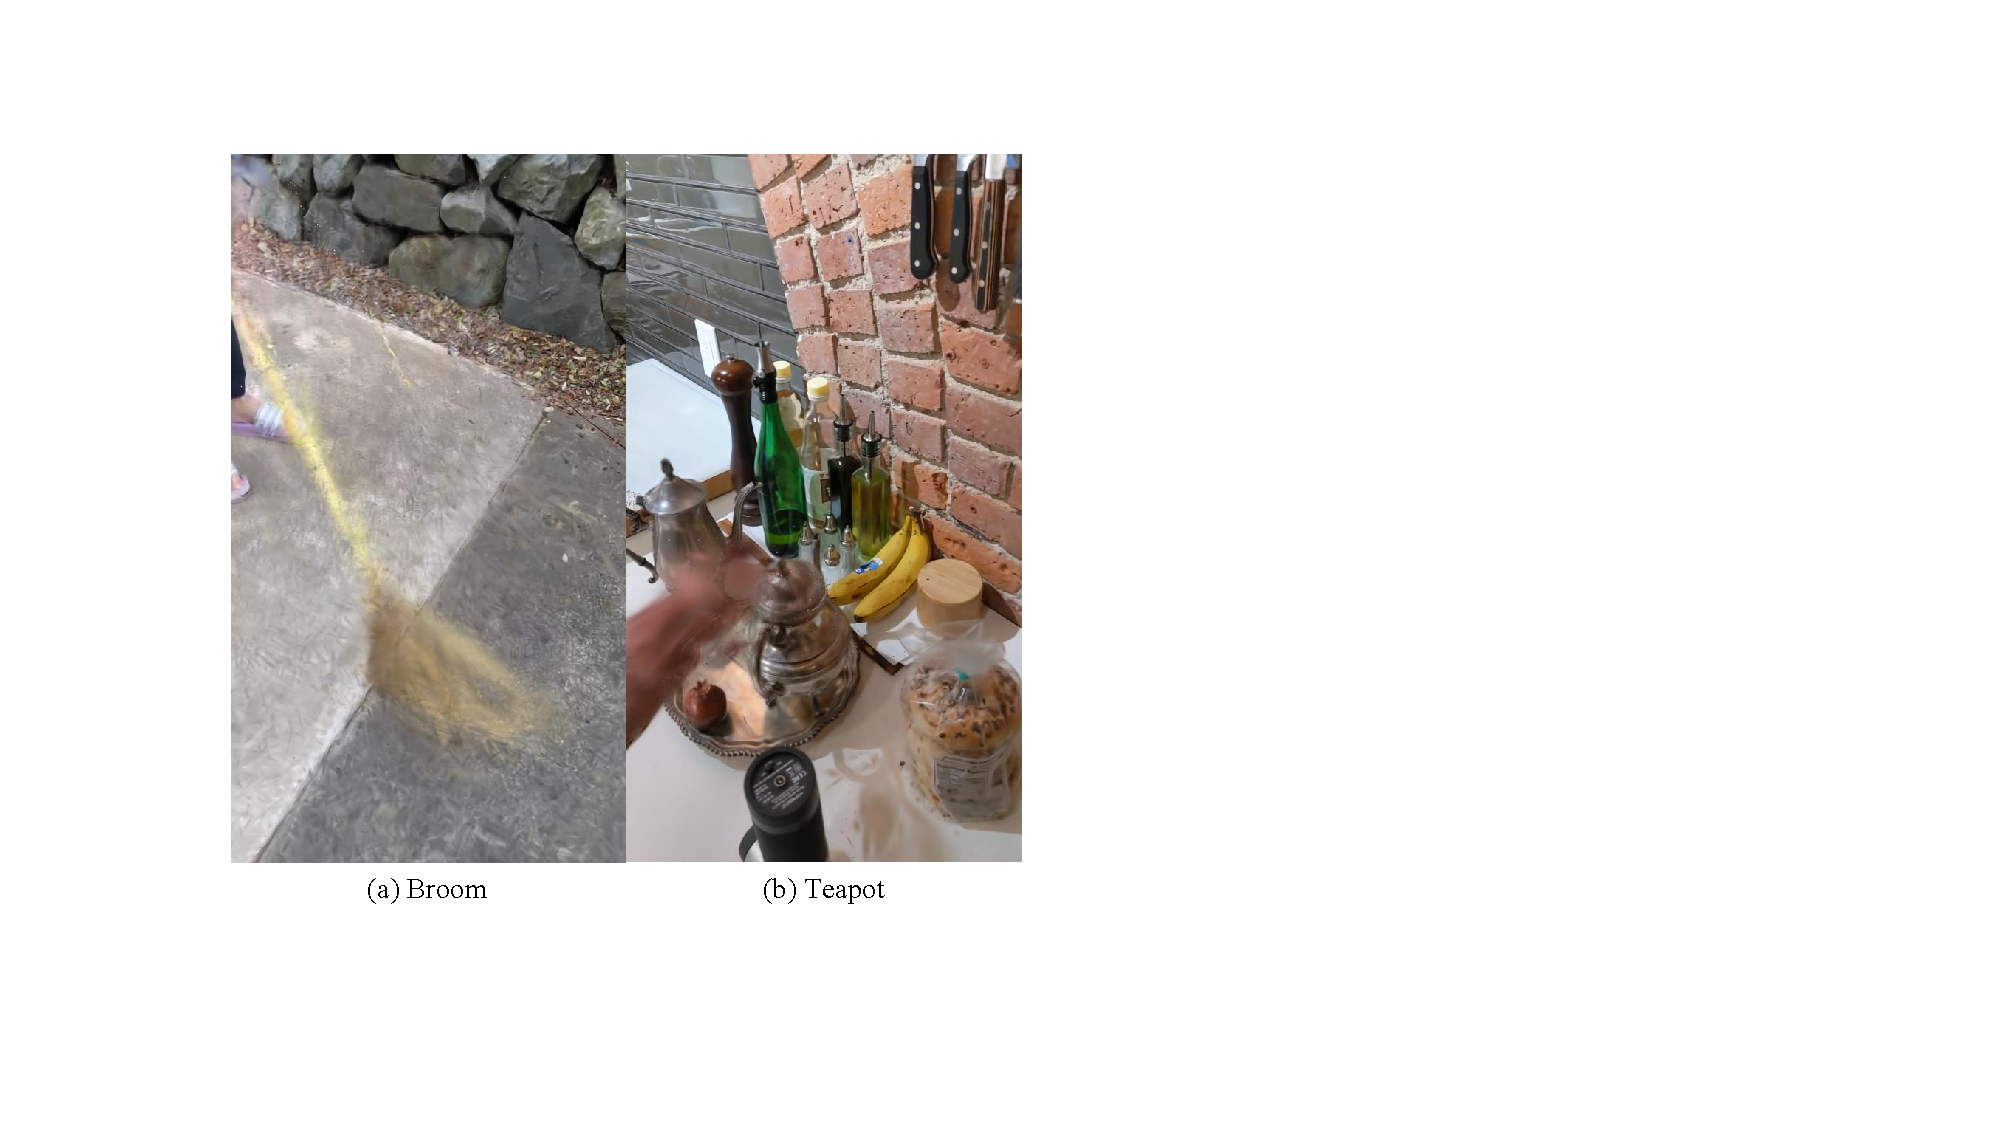
\includegraphics[width=1.0\linewidth]{fig/failurecases.pdf}
   \caption{Failure cases of modeling large motions and dramatic scene changes. (a) The sudden motion of the broom makes optimization harder. (b) Teapots have large motion and a hand is entering/leaving the scene.}
    \label{fig:failurecases}
\end{figure}


\begin{table*}	
\centering  
% \fontsize{6.5}{8}\selectfont  
\begin{threeparttable}  
\caption{Perscene results of HyperNeRF's vrig datasets~\cite{park2021hypernerf} by different models.}  
\label{tab:hypernerf_comparison}  
\begin{tabular}{l|cc|cc|cc|cc}  
\toprule  
\multirow{2}{*}{Method}&  
\multicolumn{2}{c}{3D Printer}&\multicolumn{2}{c}{Chicken}&\multicolumn{2}{c}{Broom}&\multicolumn{2}{c}{Banana}\cr  
\cmidrule(lr){2-3}\cmidrule(lr){4-5}\cmidrule(lr){6-7}\cmidrule(lr){8-9}
&PSNR&MS-SSIM&PSNR&MS-SSIM&PSNR&MS-SSIM&PSNR&MS-SSIM\cr  
\midrule  
Nerfies~\cite{park2021nerfies}&20.6&0.83&26.7&0.94&19.2&0.56&22.4&0.87\cr  HyperNeRF~\cite{park2021hypernerf}&20.0&0.59&26.9&0.94&19.3&0.59&23.3&0.90\cr  
TiNeuVox-B~\cite{tineuvox}&\cellcolor{pink}22.8&\cellcolor{pink}0.84&\cellcolor{yellow}28.3&\cellcolor{pink}0.95&21.5&0.69&24.4\cellcolor{yellow}&\cellcolor{yellow}0.87\cr  
FFDNeRF~\cite{guo2023forwardflowfornvs}&\cellcolor{yellow}22.8&\cellcolor{yellow}0.84&28.0&\cellcolor{yellow}0.94&21.9\cellcolor{yellow}&0.71\cellcolor{pink}&24.3&0.86\cr
3D-GS~\cite{3dgs}&18.3&0.60&19.7&0.70&20.6&0.63&20.4&0.80\cr
Ours&22.1&0.81&\cellcolor{pink}28.7&0.93&\cellcolor{pink}22.0&0.70\cellcolor{yellow}&\cellcolor{pink}28.0&\cellcolor{pink}0.94\cr
\bottomrule  
\end{tabular}  
\end{threeparttable}  
\end{table*}  


\begin{table*}
\centering  
% \fontsize{6.5}{8}\selectfont  
\begin{threeparttable}  
\caption{Per-scene results of DyNeRF's~\cite{li2022neural} datasets.}  
\label{tab:dynerf_comparison}  
\begin{tabular}{l|cc|cc|cc}  
    \toprule  
    \multirow{2}{*}{Method}&  
    \multicolumn{2}{c}{Cut Beef}&\multicolumn{2}{c}{Cook Spinach}&\multicolumn{2}{c}{Sear Steak}\cr  
    \cmidrule(lr){2-3}\cmidrule(lr){4-5}\cmidrule(lr){6-7}
    &PSNR&SSIM&PSNR&SSIM&PSNR&SSIM\cr  
    \midrule  
    NeRFPlayer~\cite{song2023nerfplayer}&31.83&0.928&32.06&0.930&32.31&0.940\cr
    HexPlane~\cite{hexplane}&\cellcolor{yellow}32.71&\cellcolor{pink}0.985&31.86&\cellcolor{pink}0.983&32.09&0.986\cr
    KPlanes~\cite{kplanes}&31.82&0.966&\cellcolor{pink}32.60&\cellcolor{yellow}0.966&\cellcolor{pink}32.52&\cellcolor{pink}0.974\cr
    MixVoxels~\cite{wang2023mixedvoxels}&31.30&0.965&31.65&0.965&31.43&\cellcolor{yellow}0.971\cr
    Ours&\cellcolor{pink}32.90&0.957&\cellcolor{yellow}32.46&0.949&\cellcolor{yellow}32.49&0.957\cr
\toprule  
    \multirow{2}{*}{Method}&  
    \multicolumn{2}{c}{Flame Steak}&\multicolumn{2}{c}{Flame Salmon}&\multicolumn{2}{c}{Coffee Martini}\cr  
    \cmidrule(lr){2-3}\cmidrule(lr){4-5}\cmidrule(lr){6-7}
    &PSNR&SSIM&PSNR&SSIM&PSNR&SSIM\cr  
    \midrule
    NeRFPlayer~\cite{song2023nerfplayer}&27.36&0.867&26.14&0.849&\cellcolor{pink}32.05&\cellcolor{pink}0.938\cr
    HexPlane~\cite{hexplane}&31.92&\cellcolor{pink}0.988&\cellcolor{yellow}29.26&\cellcolor{pink}0.980&-&-\cr
    KPlanes~\cite{kplanes}&32.39&0.970&\cellcolor{pink}30.44&\cellcolor{yellow}0.953&29.99\cellcolor{yellow}&\cellcolor{yellow}0.953\cr
    MixVoxels~\cite{wang2023mixedvoxels}&31.21&\cellcolor{yellow}0.970&29.92&0.945&29.36&0.946\cr
    Ours&\cellcolor{pink}32.51&0.954&29.20&0.917&27.34&0.905\cr
    \bottomrule  
\end{tabular}  
\end{threeparttable}  
\end{table*}  

\begin{table*}
\centering  
\scalebox{0.9}{

% \fontsize{6.5}{8}\selectfont  
\begin{threeparttable}  
\caption{Per-scene results of synthesis datasets.}  
\label{tab:dnerf_comparison}  
\begin{tabular}{l|ccc|ccc|ccc|ccc}  
    \toprule  
    \multirow{2}{*}{Method}&  
    \multicolumn{3}{c}{Bouncing Balls}&\multicolumn{3}{c}{Hellwarrior}&\multicolumn{3}{c}{Hook}&\multicolumn{3}{c}{Jumpingjacks}\cr  
    \cmidrule(lr){2-4}\cmidrule(lr){5-7}\cmidrule(lr){8-10}\cmidrule(lr){11-13}
    &PSNR&SSIM&LPIPS&PSNR&SSIM&LPIPS&PSNR&SSIM&LPIPS&PSNR&SSIM&LPIPS\cr  
    \midrule  
    3D-GS~\cite{3dgs}&23.20&0.9591&0.0600&24.53&0.9336&0.0580\cellcolor{yellow}&21.71 & 0.8876& 0.1034& 23.20&0.9591 &0.0600\cr  
    K-Planes\cite{kplanes}&40.05&\cellcolor{yellow}0.9934&0.0322\cellcolor{yellow}&24.58&0.9520&0.0824&28.12&0.9489&0.0662&31.11&0.9708&0.0468\cr  
    HexPlane\cite{hexplane}&39.86&0.9915&0.0323&24.55&0.9443&0.0732&28.63&0.9572\cellcolor{yellow}&0.0505\cellcolor{yellow}&31.31&0.9729&0.0398\cr  
    TiNeuVox\cite{tineuvox}&\cellcolor{yellow}40.23&0.9926&0.0416&\cellcolor{yellow}27.10&\cellcolor{yellow}0.9638&0.0768&28.63\cellcolor{yellow}&0.9433&0.0636&33.49\cellcolor{yellow}&0.9771\cellcolor{yellow}&0.0408\cellcolor{yellow}\cr  		Ours&\cellcolor{pink}40.62&\cellcolor{pink}0.9942&\cellcolor{pink}0.0155&\cellcolor{pink}28.71&\cellcolor{pink}0.9733&\cellcolor{pink}0.0369&\cellcolor{pink}32.73&\cellcolor{pink}0.9760&\cellcolor{pink}0.0272&\cellcolor{pink}35.42&\cellcolor{pink}0.9857&\cellcolor{pink}0.0128\cr  
\toprule  
\multirow{2}{*}{Method}&  
    \multicolumn{3}{c}{Lego}&\multicolumn{3}{c}{Mutant}&\multicolumn{3}{c}{ Standup}&\multicolumn{3}{c}{Trex}\cr  
    \cmidrule(lr){2-4}\cmidrule(lr){5-7}\cmidrule(lr){8-10}\cmidrule(lr){11-13}
    &PSNR&SSIM&LPIPS&PSNR&SSIM&LPIPS&PSNR&SSIM&LPIPS&PSNR&SSIM&LPIPS\cr  
    \midrule  
    3D-GS~\cite{3dgs}&23.06&0.9290&0.0642&20.64&0.9297&0.0828&21.91&0.9301&0.0785&21.93&0.9539&0.0487\cr  
    K-Planes~\cite{kplanes}&\cellcolor{pink}25.49&\cellcolor{pink}0.9483&\cellcolor{pink}0.0331&32.50&0.9713&0.0362&33.10&0.9793&0.0310&30.43&0.9737&0.0343\cr  
    HexPlane~\cite{hexplane}&\cellcolor{yellow}25.10&\cellcolor{yellow}0.9388&0.0437&33.67\cellcolor{yellow}&0.980\cellcolor{yellow}2&0.0261\cellcolor{yellow}&34.40&\cellcolor{yellow}0.9839&\cellcolor{yellow}0.0204&30.67&\cellcolor{yellow}0.9749&\cellcolor{yellow}0.0273\cr  
    TiNeuVox~\cite{tineuvox}&24.65&0.9063&0.0648&30.87&0.9607&0.0474&\cellcolor{yellow}34.61&0.9797&0.0326&\cellcolor{yellow}31.25&0.9666&0.0478\cr  
    Ours&25.03&0.9376&0.0382\cellcolor{yellow}&\cellcolor{pink}37.59&\cellcolor{pink}0.9880&\cellcolor{pink}0.0167&\cellcolor{pink}38.11&\cellcolor{pink}0.9898&\cellcolor{pink}0.0074&\cellcolor{pink}34.23&\cellcolor{pink}0.9850&\cellcolor{pink}0.0131\cr  
    % B&0.7667&0.7644&0.7646&0.6609&0.6687&0.6574\cr  
    % A&{\bf 0.8189}&{\bf 0.8139}&{\bf 0.8146}&{\bf 0.6971}&{\bf 0.6904}&{\bf 0.6935}\cr  
    \bottomrule  
\end{tabular}  
\end{threeparttable}  
}
\end{table*}  


\begin{table}
\centering  
% \fontsize{6.5}{8}\selectfont  
\caption{Ablation Study on $\phi_{\mathcal{C}}$ and $\phi_{\mathcal{\alpha}}$, comparing with TiNeuVox~\cite{tineuvox} in Americano of HyperNeRF~\cite{park2021hypernerf}'s dataset.}
\begin{threeparttable}  
\label{tab:ablation_dshsdo}  
\begin{tabular}{l|cc }  
\toprule  
\multirow{2}{*}{Method}&  
\multicolumn{2}{c}{Americano}\cr  
\cmidrule(lr){2-3}
&PSNR&MS-SSIM\cr  
\midrule  
TiNeuVox-B~\cite{tineuvox}&28.4&0.96\cr  
Ours w/ $\phi_{\mathcal{C}}$,$\phi_{\mathcal{\alpha}}$ &\cellcolor{pink}31.53&\cellcolor{pink}0.97\cr
Ours&\cellcolor{yellow}30.90&\cellcolor{yellow}0.96\cr
\bottomrule  

\end{tabular}  
\end{threeparttable}  
\label{table:ab_dshsdo}

\end{table}  
\appendix

\section{Appendix}

\subsection{Introduction}
In the supplementary material, we mainly introduce our hyperparameter settings of experiments in Sec.~\ref{Supsec:hyperparameters}. Then more ablation studies are conducted in Sec.~\ref{Supsec:ablationstudies}. Finally, we delve into the limitations of our proposed 4D-GS in Sec.~\ref{supsec:discussions}.


\subsection{Hyperparameter Settings}
\label{Supsec:hyperparameters}
Our hyperparameters mainly follow the settings of 3D-GS~\cite{3dgs}. The basic resolution of our multi-resolution HexPlane module $R(i,j)$ is set to 64, which is upsampled by 2 and 4. The learning rate is set as $1.6\times10^{-3}$, decayed to $1.6e-4$ at the end of training. The Gaussian deformation decoder is a tiny MLP with a learning rate of $1.6\times10^{-3}$ which decreases to $1.6\times10^{-3}$. The batch size in training is set to 1. The opacity reset operation in \cite{3dgs} is not used as it does not bring evident benefit in most of our tested scenes. Besides, we find that expanding the batch size will indeed contribute to rendering quality but the training cost increases accordingly.

Different datasets are constructed under different capturing settings. D-NeRF~\cite{pumarola2021dnerf} is a synthesis dataset in which each timestamp has only one single captured image following the monocular setting. This dataset has no background which is easy to train, and can reveal the upper bound of our proposed framework. We change the pruning interval to 8000 and only set a single upsampling rate of the multi-resolution HexPlane Module $R(i,j)$ as 2 because the structure information is relatively simple in this dataset. The training iteration is set to 20000 and we stop 3D Gaussians from growing at the iteration of 15000.

The DyNeRF dataset~\cite{li2022neural} includes 15 -- 20 fixed camera setups, so it's easy to get the sfm~\cite{schonberger2016structurefrommotion} point in the first frame, we utilize the dense point-cloud reconstruction and downsample it lower than 100k to avoid out of memory error. Thanks to the efficient design of our 4D Gaussian splatting framework and the tiny movement of all the scenes, only 14000 iterations are needed and we can get the high rendering quality images. 
% The visualization of our model is shown in Fig.~\ref{fig:dynerf_result_vis}.

HyperNeRF's dataset is captured with less than 2 cameras in feed-forward settings. We change the upsampling resolution up to $[2,4]$ and the hidden dim of the decoder into 256. Similar to other works~\cite{tineuvox,park2021hypernerf}, we found that Gaussian deformation fields always fall into the local minima that link the correlation of motion between cameras and objects even with static 3D Gaussian initialization. And we're going to reserve the splitting of the relationship in the future works. 
% The visualization of our model is shown in Fig.~\ref{fig:hypernerf_result_sup}.

\subsection{More Ablation Studies}
\label{Supsec:ablationstudies}
\paragraph{Position Deformation.} We find that removing the output of the position deformation head can also model the object motion. It is mainly because leaving some 3D Gaussians in the dynamic part, keeping them small in shape, and then scaling them up at a certain timestamp can also model the dynamic part. However, this approach can only model coarse object motion and lost potential for tracking. The visualization is shown in Fig.~\ref{fig:no_dx_vis}.
\paragraph{Editing with 4D Gaussians.}
We provide more visualization in editing with 4D Gaussians with Fig.~\ref{fig:editing_supp}.  This work only proposes a naive approach to transformation. It is worth noting that when applying the rotation of the scenes, 3D Gaussian's rotation quaternion $q$ and scaling coefficient $s$ need to be considered. Meanwhile, some interpolation methods should be applied to enlarge or reduce 4D Gaussians.
\paragraph{Color and Opacity's Deformation.}
When encountered with fluid or non-rigid motion, we adopt another two output MLP decoder $\phi_{\mathcal{C}}$, $\phi_\alpha$ to compute the deformation of 3D Gaussian's color and opacity $\Delta \mathcal{C} = \phi_{\mathcal{C}}(f_d)$, $\Delta \alpha = \phi_{\mathcal{\alpha}}(f_d)$. Tab.~\ref{table:ab_dshsdo} and Fig.~\ref{fig:ab_dshs} show the results in comparison with TiNeuVox~\cite{tineuvox}. However, it is worth noting that modeling Gaussian color and opacity change may cause irrational shape changes when rendering novel views. \ie the Gaussians on the surface should move with other Gaussians but stay in the place and the color is changed, making the tracking difficult to achieve.
\paragraph{Spatial-temporal Structure Encoder.}
We have explored why 4D-GS can achieve such a fast convergence speed and rendering quality. As shown in Fig.~\ref{fig:grid_feature_vis_supp}, we visualize the full features of $R_1$ in bouncingballs. It's explicit that in the $R_1(x,y)$ plane, the spatial structure of the scenes is encoded. Similarily, $R_1(x,z)$ and $R_1(y,z)$ also show different view structure features. Meanwhile, temporal voxel grids $R_1(x,t),R_1(y,t)$ and $R_1(z,t)$ also show the integrated motion of the scenes, where large motions always stand for explicit features. So, it seems that the proposed HexPlane module encodes the features of spatial and temporal information.


\subsection{More Discussions}
\label{supsec:discussions}
\paragraph{Monocular Dynamic Scene Reconstruction.}
In monocular settings, input data are sparse from both cameration pose and timestamp dimensions. This may cause the local minima of overfitting with training images in some complicated scenes. As shown in Fig.~\ref{fig:dycheck_supp}, though 4D-GS can render relatively high quality in the training set, the strong overfitting effects of the proposed model cause the failure of rendering novel views. To solve the problem, more priors such as depth supervision or optical flow may be needed.

\paragraph{Large Motion Modeling with Multi-Camera Settings.}
In the DyNeRF~\cite{li2022neural}'s dataset, all the motion parts of the scene are not very large and the multi-view camera setup also provides a dense sampling of the scene. That is the reason why 4D-GS can perform a relatively high rendering quality. However, in large motion such as sports datasets~\cite{joo2015panopticstudio} used in~\cite{dynamic3dgs}, 4DGS cannot fit well within short times as shown in Fig.~\ref{fig:sports_supp}. Online training~\cite{dynamic3dgs,abou2022particlenerf} or using information from other views like~\cite{lin2023im4d,wang2021ibrnet} could be a better approach to solve the problem with multi-camera input.

\paragraph{Large Motion Modeling with Monocular Settings.}
4D-GS uses a deformation field network to model the motion of 3D Gaussians, which may fail in modeling large motions or dramatic scene changes. This phenomenon is also observed in previous NeRF-based methods~\cite{tineuvox,pumarola2021dnerf,park2021hypernerf,li2022neural}, producing blurring results. Fig.~\ref{fig:failurecases} shows some failed samples. Exploring more useful priors could be a promising future direction.

% also needs sufficient training strategies. In some cases such as large and sudden motion like broom or teapot in Fig.~\ref{fig:failurecases}, 4D-GS struggles to render time-aware sequential images, making novel views \textbf{splitting} instead of \textbf{blurring} previous NeRF-based methods~\cite{tineuvox,pumarola2021dnerf,park2021hypernerf,li2022neural}.

% {
%     \small
%     \bibliographystyle{ieeenat_fullname}
%     \bibliography{main}
% }
% \end{document}


